\documentclass[10pt]{IEEEtran}
\usepackage[T1]{fontenc}
%\documentclass[12pt]{Article}
%\renewcommand\rmdefault{phv}
%\usepackage[doublespacing]{setspace}
%\usepackage[margin=1in]{geometry}
\usepackage{hyperref}
\usepackage{graphicx}
\usepackage[fleqn]{amsmath}
\usepackage{blindtext}
\usepackage{pgfplots}
\pgfplotsset{compat=1.9}
\usepackage{hyperref}
\usepackage{breakurl}
\usepackage{indentfirst}
\usepackage{authblk}
\PassOptionsToPackage{bookmarks=false}{hyperref}
\hypersetup{draft}
\usepackage{todonotes}
\usepackage{svg}
\usepackage{textcomp}
\usepackage{algorithmicx}
\usepackage[noend]{algpseudocode}
\usepackage{algorithm}
\newcommand*\Let[2]{\State #1 $\gets$ #2}
\newcommand*\Append[2]{\State #1$.append($#2$)$}
\providecommand{\myceil}[1]{\left \lceil #1 \right \rceil }
\tikzset{declare function={Ceil(\x)=round(\x+0.5);}}
\usepackage[backend=biber]{biblatex}
\addbibresource{ZTree.bib}

\title{Work in Progress: A Novel Range-Queryable Distributed Data Structure}
\author{Charles Noyes \\ cnoyes@usc.edu}
\date{\vspace{-5ex}}

\begin{document}

\maketitle

\begin{abstract}
We present the design of a novel data structure. We aim to solve the issue of window/range-based queries of distributed data stores in peer to peer architectures. Traditional models, for example, distributed hash tables (DHTs), are hostile towards window queries because their hashing operations are designed to uniformly distribute stored data across a defined key space; the hashing operations used to achieve this even key distribution inherently erases all characteristics of the target data that could be used to classify it. We solve this problem of erasure by defining a scheme in which higher-order data is mapped to a first-dimensional key space, while preserving locality. The resulting key space is not uniformly distributed, so we define a distributed consensus protocol in which participants in our network agree to target highly populated regions of the key space. This consensus scheme also provides some protection from Sybil attacks, as it is a to hash-based proof of work system. Finally, we define storage, lookup, and deletion operations that utilize balanced search trees to efficiently perform necessary network functions. A peer to peer communication system acts as the underlying network for participants, providing all of the traditional benefits of a P2P architecture.
\end{abstract}


\section{Notation}

\noindent Tuples/Lists: $[a,b,c,...]$

\noindent Application of a function $f$ to an input $x$: $y=f(x)$

\noindent Application of a hash function $H$ with $k$ output bits: $H_{k}(x) = \{0,1\}^{[k]}$

\noindent Keys of user $j$: $ PUBK_j; PRIVK_j $

 
\section{Introduction}
\par Distributed hash tables are currently one of the hottest topics in the cryptography space~\cite{Stoica:2001dj,Rowstron:2001ea,Ratnasamy:2001wn}. They are used in many large scale open sources projects~\cite{Freitas:2013tb,Xu:2010vs,Perfitt:2010fh} as their underlying infrastructure. First, in order to better understand the motivation behind this project, a brief explanation of the workings of a distributed has table (DHT) and its constituent protocols is needed.

\par Simply put, DHTs were created to provide hash table-like functionality on an Internet-scale level~\cite{Ratnasamy:2001wn}. They expose basic PUT and GET requests (operating on (key,value) pairs) to clients, allowing them to store and retrieve information from the DHT. The difference between a hash table and a DHT is the scope of the mechanism: DHTs are able to operate in an entirely decentralized setting, in which the responsibility for the mapping of keys to values is distributed pseudo-uniformly among all participants in a P2P network. Notable networks that utilize DHTs include the Coral Content Distribution Network~\cite{Freedman:2004vb}, the Storm Botnet~\cite{Holz:2008uk}, and the BitTorrent file sharing protocol~\cite{Cohen:y1_8mBnw}.

\par Keys used in traditional DHTs are calculated through the use of a hash function. Given that the digest (output) of a hash function is some number of bits, each of which has the same probability of being set to $'1'$ or $'0'$, we can confidently conclude that the outputs will be randomly distributed along the hash function's key space~\cite{Stoica:2001dj}. This keyspace is the set of all possible outputs; for a hash function with $k$ output bits, this is the set $\{0,1\}^k$. This is useful to users in a DHT because, assuming that a given hash function is 'sound,' in that its outputs are actually evenly distributed, they are able to mathematically verify the even partitioning of the key space. The participants can thus trust that the load will be balanced fairly among all nodes. No one node will have complete control, and no group of nodes will be unfairly burdened due to their residing in some supposed 'hotspots' in the key space, in which a disproportionally high number of objects are stored.

\par One important continuity between all of these examples is the use of a DHT in an 'exact-match' lookup scenario; the even distribution of hash functions once again comes into play. The purging of any locality (that is, the property of alike object's digests being somehow as 'distant' from one another as the objects themselves) precludes the possibility of range or window-based queries. Ramabhadran et al. put it very well: \textit{"However, range queries, asking for all objects with values in a certain range, are particularly difficult to implement in DHTs. This is because DHTs use hashing to distribute keys uniformly and so can't rely on any structural properties of the key space, such as an ordering among keys"}~\cite{Ramabhadran:2004tr}\textit{.}

The idea of locality vs. evenness is fundamental to our work, and so we define it here. Intuitively, we can say that locality is preserved for any given set of objects (serializable to a numeric representation in some fashion) $A,B,$ and $C$ in a function $f$ such that
\begin{equation} \label{eq:locality}
|A-B| < |B-C| \Rightarrow |f(A)-f(B)| < |f(B) - f(C)|,
\end{equation}
and garden variety hash functions obviously do not fulfill this requirement.

\section{Related Work}
\par Some research has been done on the usage of a DHT as an overlay on top of a traditional data structure to enable range queries~\cite{Ramabhadran:2004tr,Desnoyers:2008uo}, however none of the currently proposed solutions are useful in a true P2P network. Sybil attacks are arguably the most severe vulnerability in most decentralized networks~\cite{Douceur:2002jr}, with a litany of papers having been published on this attack in the context of DHTs~\cite{LesniewskiLass:2010ue}, and yet the subject is not even broached. To summarize the cited papers, Sybil attacks are executed through the undermining or subversion of reputation or voting systems through the forging of a identities in peer to peer networks.

\par Given that if we replace the cryptographic hash function in a DHT with a locality sensitive function~\footnote{Locality sensitive hash functions (LSHs) do exist, however we believe that a lower level function, such as a generic space filling curve, would be better suited for our purposes. LSHs are generally useful only in an extremely narrow set of cases.}, the distribution of keys along the key space will not be even, and so we must design a scheme by which nodes can coalesce onto the more populated areas. This is a necessity because of load balancing concerns in the context of the possibility of the defined Sybil attacks.

\par The Squid~\cite{Schmidt:2003cd}, another tangentially related project, has actually tried to define protocols for more generalized searching (e.g. range and keyword queries), in much the same way that we will. The similarities end in the applicability of their work to situations that are not just distributed in a peer to peer network, but truly decentralized. The differences between the two are slight but of paramount importance, both ideologically and practically, to the applicability of a protocol that satisfies only the first.

\par A DHT that satisfies all of these requirements would be extremely helpful to users in a variety of settings. To be clear, no other data structure in existence has these capabilities. In fact, this work is the direct result of an inability to find an existing solution. Some potential applications include:



\section{Our Approach}
\begin{figure}[!t]
\centering
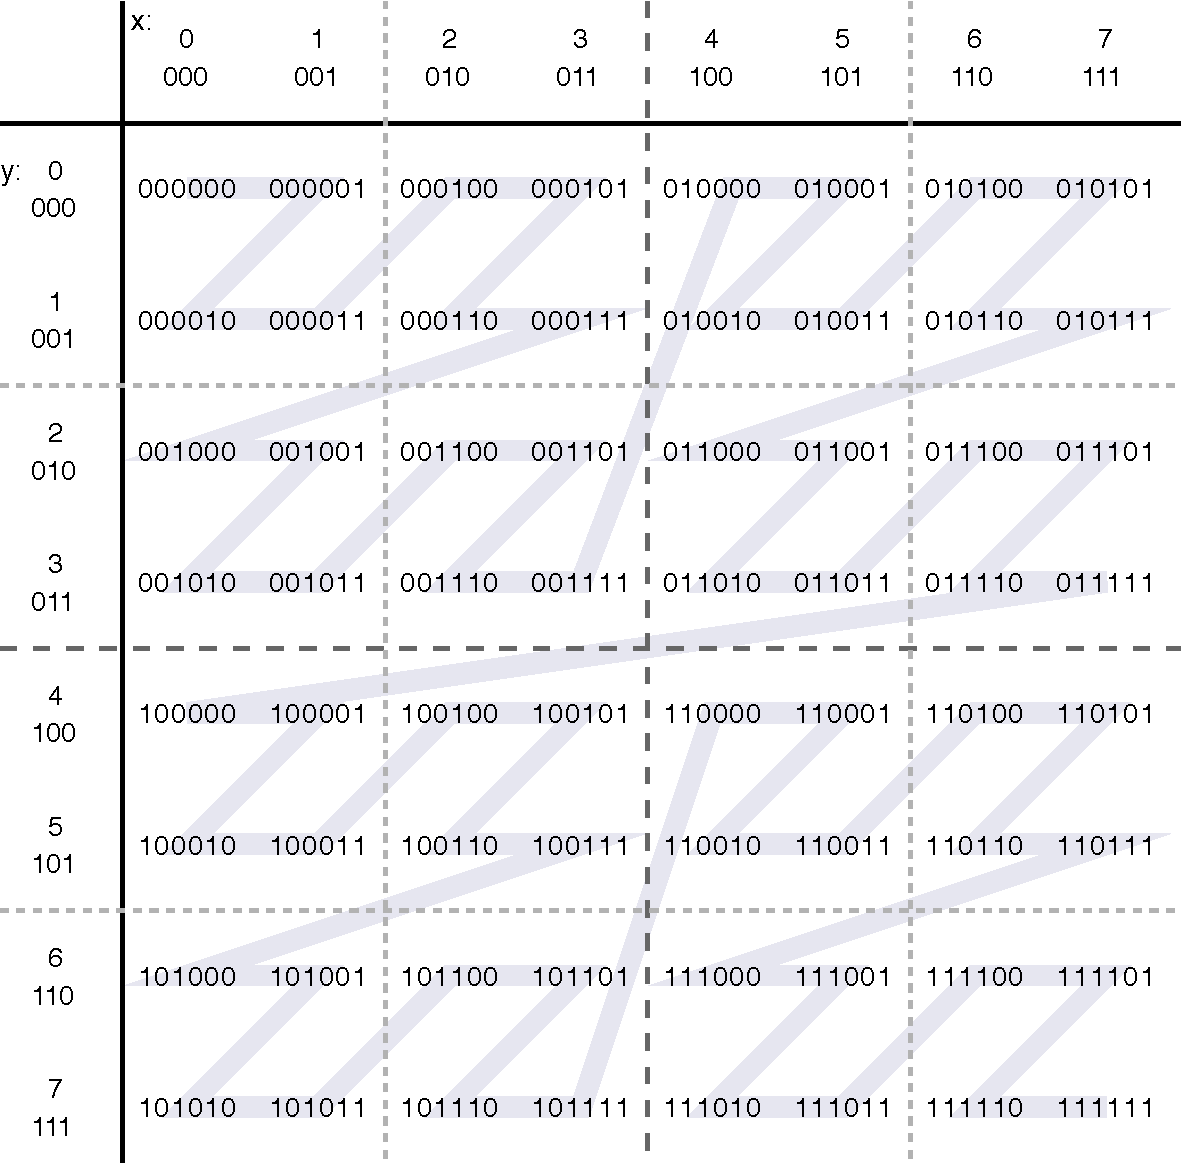
\includegraphics[width=3in]{ZCurve}
\caption{Morton Codes/Z-Order Curving~\cite{ZorderCurve:2015vo}}
\label{fig_MCode}
\end{figure}

\par We believe that the best solution is one in which we only slightly modify the way in which a DHT works. Substituting a space filling curve for a hash function would allow us to preserve locality of data in a DHT with rigorously defined limitations on what kind of data may be stored in it. A space filling curve brings its own set of limitations, however, and so we also present a method of solving these problems.

\subsection{Hash Function Replacement}

\par Currently, we believe that bit interleaving is a promising replacement for hash functions. Through the use of space filling curves, such as a Z-Order curve (sometimes called the Morton curve), $Nth$-dimensional data can be mapped to the first dimension (such that it may be stored in-memory). The mapping of a section of the integral Cartesian plane to binary, through the interleaving of the $x$ and $y$ coordinates, is illustrated in Fig.~\ref{fig_MCode}.

\par Interestingly, the interleaving of bits to form Morton codes preserves the locality of the initial data in the output, satisfying Eq.~\ref{eq:locality}. There is, however, no currently agreed upon scheme for the extension of this function to floating point numbers. A few solutions have been proposed, such as~\cite{Connor:2010eq}, but none have been truly validated. We do not believe this to be a significant obstacle, and even an imperfect solution can work for the time being.

\par For now, we are using longitudinal and latitudinal coordinates to test range based searches in a sorted key-value database. Our algorithm to serialize the decimal coordinates to bytes is as follows, where $lat$ and $lon$ are the inputs and $ZOrd$ is a bit interleaving function:

\begin{equation} \label{eq:serialization}
ZOrd(int((lat + 90) * 100), int((lon + 180) * 100))
\end{equation}

\begin{figure}[!t]
\centering
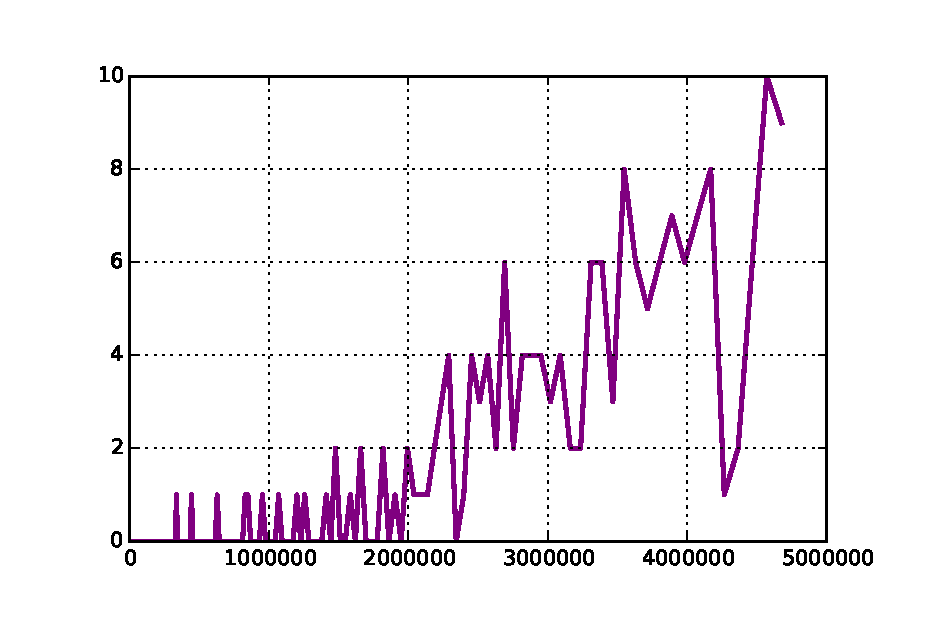
\includegraphics[width=3.5in]{errors.eps}
\caption{Bit Interleaving With A Z-Order Curve}
\label{fig_ZOrd}
\end{figure}

\par Obviously this is an imperfect solution, however the number of errors in a real-world test of this algorithm showed that the error rate is fairly negligible. To measure lookup accuracy on a large corpus, we performed a range query (note: the range was always the same) on data sets of varying sizes, using \ref{eq:serialization} as our serialization scheme.
% \begin{algorithm}
%   \begin{algorithmic}[1]
%   \Require{A '/' denotes two variables with different prefixes, and is used to save line space.}
%   \vspace{-0.4cm}
%     \Statex
%     \Function{Test}{$n,min/maxLat,min/maxLon$}
%         \Let{$storageDic$}{$\{\}$}
%         \Let{$correctResults$}{$[]$}
%         \Let{$realResults$}{$[]$}
%         \For{$i \textrm{ in Range}(n)$}
%             \Let{$lat$}{$\textrm{RandFloat}(-90,90)$}
%             \Let{$lon$}{$\textrm{RandFloat}(-180,180)$}
%             \Let{$key$}{$Eq.$~\ref{eq:serialization}$(lat,lon)$}
%             \Let{$storageDic[key]$}{$i$}
%             \If{$(minLat<lat<maxLat)\&\&$ \par 
%             \hskip\algorithmicindent$(minLon<lon<maxLon)$}
%                 \Append{$correctResults$}{$i$}
%             \EndIf
%         \EndFor
%         \Let{$minCode$}{$Eq.~\ref{eq:serialization}(minLat/Lon)$}
%         \Let{$maxCode$}{$Eq.~\ref{eq:serialization}(maxLat/Lon)$}
%         \For{$key \textrm{ in } storageDic.keys()$}
%             \If{$minCode < key < maxCode$}
%                 \Append{$realResults$}{$key$}
%             \EndIf
%         \EndFor
%         \State \Return{$len(correctResults - realResults)$}
        
%     \EndFunction
%   \end{algorithmic}
% \end{algorithm}

\par Our results are shown in Fig.~\ref{fig_ZOrd}. We are confident that this decimal flooring scheme will effectively bridge the gap of time between the work we are doing here and the validation of a floating point-ready Z-Ordering scheme.

\begin{figure}[!t]
\centering
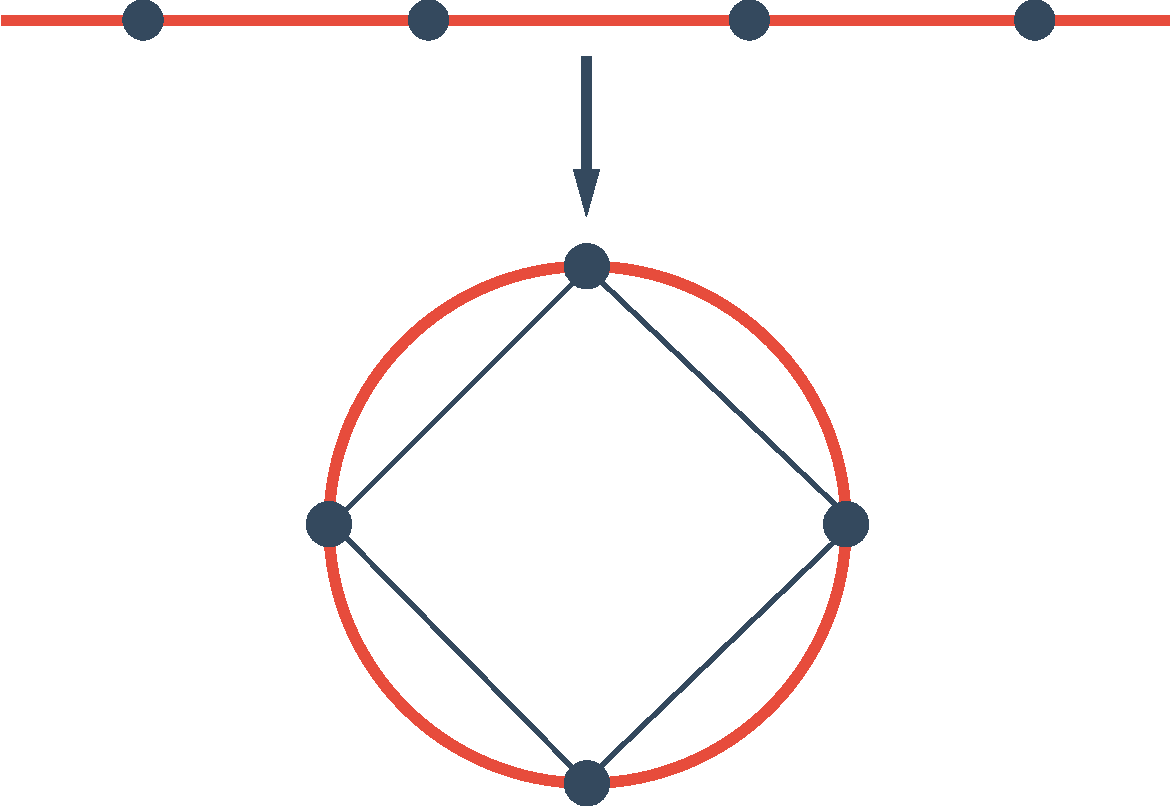
\includegraphics[width=3.5in]{finalRing}
\caption{Evenly Distributed Key Space Mapping}
\label{fig_kSpace}
\end{figure}

\subsection{Node Rearrangement}
\par Next, we come to the problem of key space distribution. Illustrated in Fig.~\ref{fig_kSpace} is the way in which we transform the linear version of the key space into a circular representation, and how the nodes communicate with their 'neighbors' in a DHT. On one 'end' of the linear representation is the lowest possible value (in binary, this would be the set $\{0\}^{[k]}$), and on the other is the maximum possible value ($\{1\}^{[k]}$). Notice that in both representations, the nodes are distributed evenly. Each occupies the same amount of space as the others, and together they cover the entire key space. We don't even need to populate the key space with examples, as we can prove that they will cover it evenly when using a 'good' hash function as the key function.

\par If we were to use a Z-Ordering scheme as the key space location function, we will almost certainly have the data become 'clustered' in some sense. For example, if we were to store all of the data about the global land-line network, we would most likely have all of the data from highly populated areas focused on a few regions in the key space, and oceans of nothingness between them. This is an unavoidable byproduct of the use of a locality-preserving function.



\par Fig.~\ref{fig_kSpaceUneven} shows a distributed data structure in which a locality preserving function was used, with red highlights gauging the fullness of each region in the key space. Notice that two of the nodes are doing nearly all of the work, while the others have no load to bear. There is no existing mechanism for nodes to retroactively redistribute themselves.


\par We propose the inclusion of cryptographic proof of work, ala Hashcash~\cite{Back:2002vq}, with each stored piece of data. Because these proofs are difficult to compute, no entity can easily execute a Sybil-like attack against the rest of the network by including 'junk' proofs; all others would simply be able to see that the proofs are incorrect. A user $j$ would send this to the rest of the network:

\begin{figure}[!t]
\centering
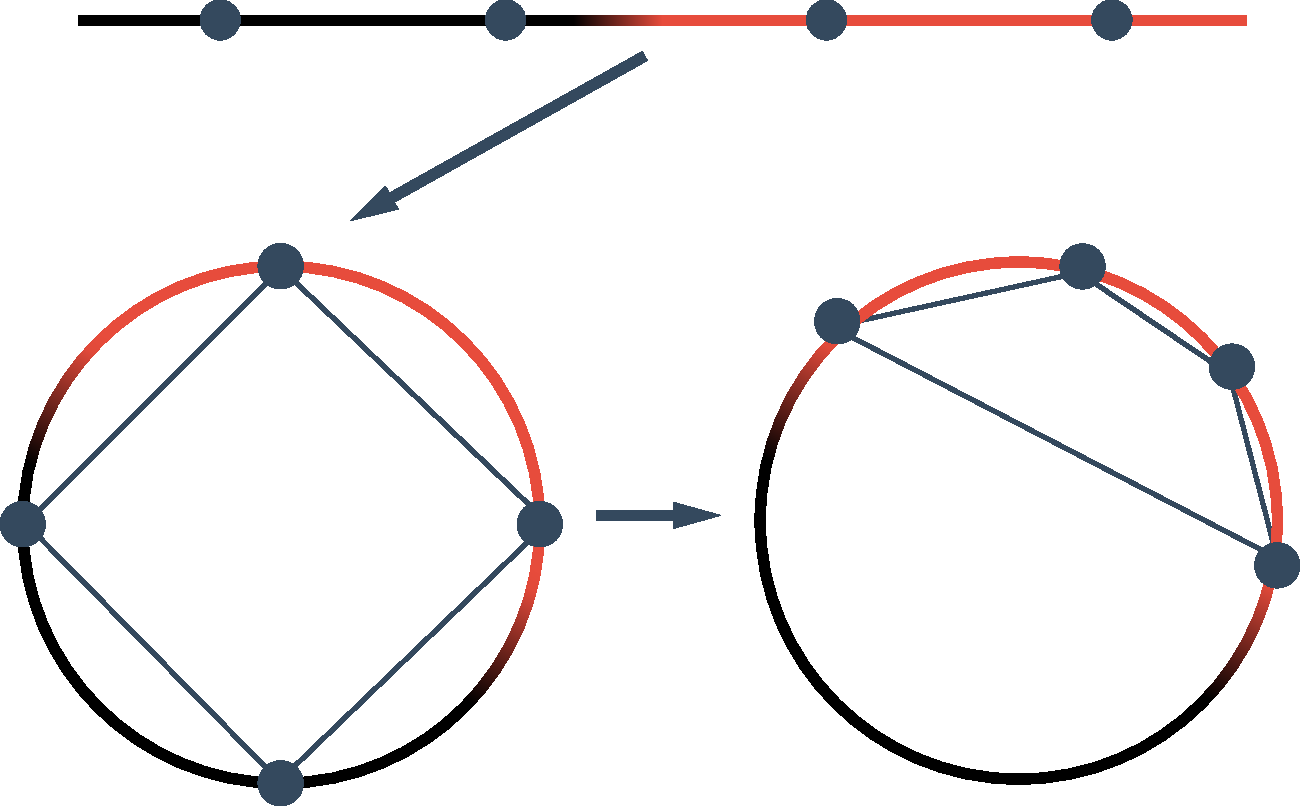
\includegraphics[width=3.5in]{unevenDistro}
\caption{Node Convergence}
\label{fig_kSpaceUneven}
\end{figure}

\begin{equation} \label{eq:proof}
SerializedData = [PrivK_{j}((H(Data)), Data, PubK_{j}]
\end{equation}

\par When the nodes in a network wish to reconfigure themselves, all nodes are instructed to report all of the proof of work they know about. All of the nodes then independently construct a curve of the key space population and attempt to converge on this region. Given that there will always be a global maxima, this is relatively trivial. The actual methodology of this convergence is the core focus of our ongoing research. Currently, we are exploring the possibility of using the derivative of the fitted curve to calculate optimal node spacing.

\par From a game theory perspective, the proof of work system is greatly beneficial. Sybil attacks are largely mitigated, and there is no obvious advantage for a malicious node to withhold its knowledge of the proofs in its region. It does, however, introduce some amount of overheard into the network. We believe that this is not a terribly inhibiting factor, as the use cases for a decentralized (i.e. public) version of our data structure are almost always either altruistic or capitalistic in nature. To give an example of the former, folding@Home~\cite{Anderson:2002vr}, a network in which people donate unused computational resources to fold proteins, has been wildly successful. Bitcoin~\cite{Nakamoto:2008ti}, the decentralized P2P cryptocurrency network, is an excellent example of hashing power being used for the latter case. In both networks, there is no lack of available resources.

\par Lastly, we are exploring the use of distributed hash chaining, such as the Bitcoin blochchain, as a mechanism to to allow for higher level consensus in our network. Twister~\cite{Freitas:2013tb} showed that it is possible to intertwine a DHT and a blockchain to allow for things like user verification and to act as a decentralized key server. Currently we are exploring the usage of a blockchain as a reporting service for the network, taking 'snapshots' of all known proofs of work at a given interval. In this way, we could be certain that all nodes would calculate their position deterministically, instead of relying on disparate levels of information.

\section{Analysis}
\subsection{Sybil Attacks on The DHT Proper}
\par Some of the claims made thus far are provable only in the abstract. For example, we assert that Sybil attacks are mitigated through a proof of work system and that this work is not a growth inhibiting factor. Our proof of work system is a basic one, modeled on the HashCash~\cite{Back:2002vq} system. We define a 'proof' as being the value resulting of the inputting of both information and a random number to a hash function. If this proof meets the threshold of difficulty set by the network, it is accepted as valid. To show this, we assume that for a hash function of k bits, the set of possible results is exactly $\{0,1\}^{[k]}$. The odds of any $k'th$ bit being $0$ or $1$ are exactly even (in this case, $1:1$). Thus, the odds of the first $n$ bits being set to 0 is exactly $\frac{1}{2^n}$. Note that simply using $0$-prefixing as the method of work determination is simplistic, and 'better' schemes (like that of Bitcoin, which uses full hex values) can provide finer control. 

\par When applied to our data structure, we would be using the number of votes as our difficulty determining factor. The difficulty should be proportionate to the number of votes and dependant on some predefined ratio of necessary goodness (generally this will be $ > 50\%$, as a result of the Byzantine general problem's theoretical limits in the general case\cite{Lamport:1982fr}). Mathematically,
\begin{multline}
N = \textrm{population size} \\
m = \textrm{proportion of wanted goodness} \\
n = \textrm{maximum difficulty} \\
q = \textrm{average number of tries} \\
z = \textrm{number of required 0 bits} \\
z = \myceil{log_2{ (\frac{2^n}{\frac{N}{m}})}}, q = 2^z \\
\end{multline}

\begin{figure}
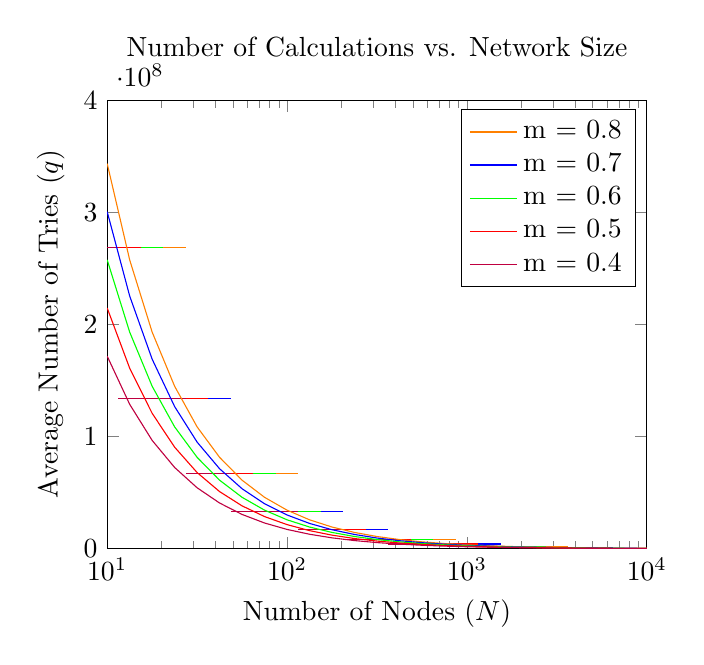
\begin{tikzpicture}
\begin{semilogxaxis}[
    jump mark mid,
    domain=10:10000,
    xmin = 10,
    xmax = 10000,
    ymin = 0,
    ymax = (0.4 * 10^9),
    title = {Number of Calculations vs. Network Size},
    xlabel = {Number of Nodes ($N$)},
    ylabel = {Average Number of Tries ($q$)},
    title style={yshift=1.5ex}
    ]
\addplot[color=orange]{2^(Ceil(ln((4294967296) / (x / 0.8))/ln(2)))};
\addplot[color=blue]{2^(Ceil(ln((4294967296) / (x / 0.7))/ln(2)))};
\addplot[color=green]{2^(Ceil(ln((4294967296) / (x / 0.6))/ln(2)))};
\addplot[color=red]{2^(Ceil(ln((4294967296) / (x / 0.5))/ln(2)))};
\addplot[color=purple]{2^(Ceil(ln((4294967296) / (x / 0.4))/ln(2)))};
\legend{m = 0.8,m = 0.7, m = 0.6,m = 0.5,m = 0.4}
\end{semilogxaxis}
\begin{semilogxaxis}[
    domain=10:10000,
    xmin = 10,
    xmax = 10000,
    ymin = 0,
    ymax = (0.4 * 10^9),
    yticklabels={,,},
    xticklabels={,,},
    hide axis
    ]
\addplot[color=orange]{(4294967296) / (x / 0.8)};
\addplot[color=blue]{(4294967296) / (x / 0.7)};
\addplot[color=green]{(4294967296) / (x / 0.6)};
\addplot[color=red]{(4294967296) / (x / 0.5)};
\addplot[color=purple]{(4294967296) / (x / 0.4)};
\end{semilogxaxis}

\end{tikzpicture}
\caption{Scaling Validation}
\label{fig_tryGraph}
\end{figure}

\par A reference graph for $n = 32$ is shown in Fig.~\ref{fig_tryGraph}, highlighting the relation between goodness thresholds ($m$) and the average number of hash calculations needed to find a good nonce (a random number) ($q$), along varying network sizes ($N$). The lines with a ceiling function applied are those that would use only $0$-bit prefixing, whereas the continuous lines are those that would use an ideal scheme (even hex values are not truly continuous, but there are many more 'steps'). Illustrated is the proof of proper scaling to large network sizes. 

\par In a network with $100,000$ participants, the number malicious 'votes' that must be cast is $ > \frac{100000}{m}$. So, when $m = 0.5$ and $n = 50$, a normal user will have to calculate (about) $560000000$ hashes to find a good nonce. Note that $n = 50$ is a more realistic baseline than $n = 32$. With a hash rate of $500KH/s$ and a wattage of of $650W$, reasonable empirical estimates of the hash rate and wattage of an average computer, it would take approximately $180$ seconds to find a nonce, or less than $1$\textcent. However, for an attack attempting to breach the consensus threshold $m$ of the network, it would take over $10,000$ hours or over $\$750$. Note that all monetary calculations assume an electricity cost of $0.12/KWh$, the national average in the U.S. according to the national Energy Information Administration.


\par One notable feature of our scheme is that the amount of power necessary to overcome the network is a constant. Because we are decreasing the amount of work required from each new vote based on the current amount, the requisite amount of power required to overcome the rest of the network is also decreased. We present this path as it is a relatively new one, and, for our planned purposes, it is likely more beneficial to lower the barrier to entry once the network becomes large. Discussed later \todo{put section here} are the ways we can combine our Sybil resistant protocols with others to chain together security. 
\par For networks that are to be used only in the short term, are large but run on devices without much computational power, or that would benefit more from a lower barrier to entry than would be allowed for with linear scaling of the hashing requirements, our scheme works best. Many autonomous networks fit this set of criteria, and for those that don't, a system where the required work is not dependant on the present work can be used. Perhaps a hybrid system, for example one in which the requisite work does not scale perfectly with the theoretical amount of work required for a Sybil attack overcoming $m$, or perhaps one in which there is a 'schedule' that the network tries to follow and which the amount of work required depends on the deviation from that schedule (more work puts us ahead of schedule, so we increase in the difficulty and vice versa) ala Bitcoin. There are really an endless number of possibilities, and our approach is presented here because no other scheme presents a viable scaled difficulty model.


\subsection{}
\section{Conclusions}
\par The end game, at least in our eyes, is a working decentralized sensornet (a sensornet being a distributed network of autonomous sensors) using our novel data structure as the method of communication. This could be anything from a disease reporting network to a climate monitoring service. Before beginning this research, we identified a need for a distributed data structure that would work under these conditions, allow for range-based querying, and be resistant to Sybil-like attacks. We are confident that this proposal presents the best avenue forwards in this space.



\printbibliography
\end{document}
